\documentclass[a4paper,12pt]{article}
\usepackage[bulgarian]{babel}
\usepackage{hyperref}
\usepackage{graphicx} 
\usepackage[margin=2.5cm]{geometry}
\usepackage{setspace}
\usepackage{float}
\usepackage{booktabs}
%opening
\title{Макроикономически последици от COVID-19 върху икономиката на България}
\date{2022-04-20}
\author{Костадин Костадинов, Светлин Ненов, Джелал Фаик}

\begin{document}

\maketitle

\setstretch{1.5}
\section{Въведение}
Началото на 2020 г. бележи нова епоха и предизвикателства, непознати досега пред световната икономика и в частност икономиката на България.

Да останат на пазара, да се адаптират към новите условия и да напаснат производствата си, са сред основните и най-трудни задачи пред всеки икономически субект. Европейският съюз успя, чрез различни лостове и механизми, да намали до минимум предприятията, обявени в несъстоятелност в резултат от пандемията. 

Въпреки усилията на държавно ниво, има установено свиване в потреблението, поне в началния етап от пандемията. През погледа на различните икономически теории пандемията може да бъде разгледана като "шок" с многофакторна генеза. Въпреки изградените модели на оценка на въздействие, все още остава отворен въпроса за механизмите на икономически отговор и предполагаемите ефекти в дългосрочен план.

\section{Литературен обзор}

В основа на литературното търсене, не би било уместно да се твърди, че COVID-19 е уникална, нова или неповторима икономическа или социална ситуация\cite{https://doi.org/10.1111/joes.12423}. 

С началото на пандемията редица автори правят аналогия с предишни вирусни епидемии. Като основен модел се приема епидемията от Испански грип 1918-1920г. \cite{barro_coronavirus_2020}. Използван, като основополагащ пункт анализите за този период установяват намаляване на реалния БВП с 6\% и намаление в потреблението с 8\%, като се прави сравнение ефектите на пандемията с тези на световната рецесия през 2008-2009г. Въпреки това следва да се подчертаят редица ограничения пред прякото имплиментиране на ефекта от Испанския грип върху очакванията ни за икономически отговор към COVID-19\cite{eichenbaum_epidemics_2020-1}. 

В анализ на Carlsson-Szlezak et al. \cite{carlsson-szlezakUnderstandingEconomicShock2020a} се описват три основни механизма на повлияване на настоящата COVID-19 пандемия върху икономическото развитие:
\begin{itemize}
	\item  На първо място чрез временно намаляване на \textbf{съвкупното търсене}. Това се обяснява в основа на наложените мерки за социална дистанция, чувството за страх от заразяване\cite{Eichenbaum2022}, препоръките за оставане по домовете и създаване на песимистични настроения за дълготрайното икономическо развитие. 
	\item  Шок от страна на \textbf{съвкупното предлагане}. Редукция в производителността на труда (поради противоепидемични препоръки, преустановяване на част от дейността в отрасъл услуги или заразяване и карантина на работниците) \cite{doi:10.1080/1540496X.2020.1785426}
    \item  Нарушен поток на доставките. Това от своя страна е следствие на временни рестрикции по отношение на свободното придвижване на факторите на производство. 
\end{itemize}

Според този модел \cite{carlsson-szlezakUnderstandingEconomicShock2020a} трите механизма действат заедно, като съотношението или преобладаващият от тях е следствие на преди всичко регионални отраслови специфики и нивото на икономическо развитие преди началото на пандемията. 

Разглеждайки механизма на икономическото въздействие, следва да се подчертае ролята на агрегирания показател на съвкупното \textbf{предлагане}. Редица са факторите водещи до намаляване в предлагането, като подобно на пандемията от Испанския грип през 1918г. като основни тригери се посочат \textit{намалената работна сила} (следствие на боледуване или преждевремена смърт), както и необходимостта от мерки намаляващи разпространението на инфекциозния процес (социална дистанция) в редица производства \cite{Frist2006} водещи и до редукция в производителността на труда. 

Следва да се подчертае, че някои автори не отъждествяват редукцията в предлагането, като директно свързан с пандемичния процес икономически ефект \cite{guerrieri_macroeconomic_2020-1}. По мнение на последните за да бъде връзката причинно-следствена, то намаляването на предлагането следва да се наблюдава в значително дълъг времеви период (поне една година), да засегне (пенетрира) повече един сектор и да е налице синхронна редукция в повече от една държава. 

За разлика от Испанския грип, тези предположения до голяма степен са валидни за пандемията от COVID-19. Причината за това е по-високото ниво на глобализация, довело до по-голяма синхронност в епидемиологичния процес и следствие на това въведените социалните и икономически мерки, налагани в различните държави\cite{barua_understanding_2021-1}. В резултат, в началото на пандемията, с налагането на най-строгите рестрикции синхронно в редица държави, се установява рязко намаляване на продуктивната сила. 

Доказателство за това са публикации от средата на 2020г., които установяват редукция на работното време (като измерим показател на производителността на труда) с повече от 40\%\cite{bloom_impact_2020-1}. Авторите установят и липса на пълно възстановяване в производителността, дори и след премахване на противоепидемичните мерки в редица държави. В допълнение намаляването и прекъсването на веригата на доставките в резултат на транспортните ограничения се посочва като мултипликативен фактор в редукцията на крайното производство \cite{GOEL2021298}.

За България, анализа на Господинова С. \cite{gospodinova_2021} също очертава подобни тенденции. Авторът разглежда период от 20 години, като установява сигнификатно намаление в относителната производителност и относителния дял на заетите. Установява се увеличена безработица особено в сектор услуги. Поставя се акцент на съвкупното \textbf{предлагане}, като дълготрайно действащ шок за разлика от този на съвкупното търсене, които се определя като временен. 

По отношение на социалния аспект на безработицата някои публикации поставят акцент на социалните неравенства. В свое проучване Alon et al. \cite{NBERw26947} установяват по-висок относителен дял на жените регистрирани като безработни спрямо мъжете в същия времеви период след началото на пандемията. Поставя се участието на жените в сектора на услугите като причина за наблюдаваната зависимост.

Въпреки категоричните си ефекти върху съвкупното предлагане, не може да се твърди, че COVID-19 пандемията е индиферентна към \textbf{съвкупното търсене} \cite{brinca2020covid}. В по-голямата част от анализите в началото на пандемията емпирично е установено свиване в потреблението. Този ефект обаче е краткотраен и заместен от промяната в потребителските предпочитания \cite{NBERw27152}. 
На следващ етап (разгара на пандемията) в потреблението се заместват луксозни стоки и услуги, транспортни разходи, екскурзии, разходи за автомобили и облекло с основни хранителни стоки и продукти от първа необходимост \cite{NBERw27432}. 

Изследователи в областта обръщат внимание и на социалните неравенства по отношение на потребителското поведение \cite{chettyEconomicImpactsCOVID19}. Установени са в по-голяма степен на редукция в потреблението на високо-доходните домакинства спрямо тези с нисък и среден доход, като редукцията в потреблението в най-слаба степен се възстановява отново сред най-високодоходната група. 

В крайните етапи на пандемията отново се наблюдава намаление в сумарното потребление. В този етап това се дължи на ефекта на комбинираната фискална и монетарна политика водеща до по-високи нива инфлация \cite{cavallo_inflation_2020-1}. От своя страна последните са пряк отговор на шоковете от страна на предлагането и търсенето, като чрез съответни мерки се цели бърз стабилизационен ефект основно чрез фискална и дълготраен ефект чрез монетарна политика \cite{zlatinov}.

Логична изглежда и тезата, изследвана от Gomperes et al. и представяща увеличени инвестиции, следствие на намалено потребление, увеличени социални трансфери и очаквана инфлация в бъдеще\cite{gompers_venture_2020-1}. 

Като специфичен икономически ефект от настоящата пандемия се посочва значителното напредване в процеса на дигитализация. Това намира и отражение в потребителското поведение, като някои изследвания установяват рязък скок в потреблението в основа на електроните стокови пазари \cite{sharma2020changing}.

В заключение COVID-19 пандемията се характеризира и с друга отличителна характеристика в сферата на икономиката на здравеопазването. По данни на Kaye A. et al. \cite{KAYE2021293} настоящата пандемията е отличителна с екцесивните разходи за болнична и извънболнична помощ, скринингови тестове, а търговските сделки свързани с ваксините засилват междунационалните социални неравества.  

\section{Цел и изграждане на икономически модел} 
Настоящето изследване се фокусира върху ефектът на COVID-19 пандемията върху краткосрочната макроикономическа ситуация в България. Изследването се ограничава в \textbf{периода на 2020 г.}. В резултат на литературния обзор, настоящият анализ и представения модел се ограничава до \textbf{съвкупното предлагане}, приемайки съвкупното търсене за временно ограничено, но без съществен ефект върху реалния темп на БВП, предвид ефекта на "заместване" на предпочитанията. Моделът възприема инфлацията за константа величина за периода, без да води сама по-себе си до редукция в потребителските възможности (PPW). Настоящият анализ възприема и за непроменена пределната склонност към потребление (MC).

Задачи и основни предположения на настоящия модел са:
\begin{enumerate}
\item Да опише ранните ефекти на COVID-19 върху реалния темп БВП на глава от населението за 2020г. по области. Основно предположение е единствено тази ситуация води до промяна на темпа на икономическото развитие. 
\item Да оцени ефекта на COVID-19 върху сектор селско стопанство, индустрия и услуги на областно ниво и да намери връзка между COVID-19 характеристики и икономическия ефект в тези сектори. Предположение на модела тук е най-ранните ефекти на пандемията засягат Българската икономика, чрез сектора на услугите предвид отрасловата и характеристика преди началото на пандемията. 
\item  Да опише и оцени ефекта на безработицата, броя на заетите на трудово правоотношение и загубените работни дни върху БВП на глава от населението по области, както и да намери асоциация на тези показатели с характеристики на пандемията.
\item Да оцени възможни областни и полови различия променящи взаимовръзката COVID-19 и макроикономическия и ефект.
\end{enumerate}

\section{Материали и методи}
Изследването използва вторичен анализ на данни. Всички данни (литературни източници, анализи и таблици и презентация на проекта) са налични в свободен достъп в \href{https://github.com/kostadinoff/macroeconomics_SU_project.git}{github}  
\subsection{Данни}

\paragraph{Икономически данни}
Икономическите данни обхващат агрегирана годишна информация в срезови вид по области и включват: списъчния състав на наетите по трудово правоотношение (коефициент 2020 към 2019 г. и темп на приръст); съотношение на коефициентите за безработица (2020 към 2019г.) и темп на приръст на безработицата; регистрирани на бюрата по труда (брой), съотношение (2020 към 2019г.) и темп на приръст на регистрираните; БВП на глава от населението в реално и номинално изражение, темпа на БВП на глава от населението за 2020г.; БВП по икономически сектори (услуги, индустрия и селско стопанство) в номинално и реално изражение и темповете на реален приръст за всеки един от тях по области и от глава от населението. 

Данните са извлечени от сайта на НСИ чрез електронния достъп на инфостат. 
\paragraph{Демографска и социална статистика}
По области и в срезов вид са извлечени данните за населението в трудоспособна възраст (15-65г.); процента на население използващо компютърни онлайн базирани услуги (за 2019 и 2020г. и разликата за периода)

\paragraph{Здравна статистика}
Предоставени от МЗ са данните за всички заразени от COVID-19 и регистрирани граждани. От този информационен масив са филтрирани данните за 2020г., като е изчислено средното ниво на заболеваемост по области. Предположение в модела е че всеки заразен е бил в 14 дневна карантина. На базата на това предположение са изчислени броя загубени работни дни на 1000 души население и съотношението на загубените работни дни към общия брой работни дни за 2020г. (250 дни)

\subsection{Методи}
Използвани са статистически методи на описателна статистика (за количествените признаци в средна стойност и стандартно отклонение) а за качествените относителен дял.

Моделирането на данните се осъществява с методи на линейна регресия (OLS estimator), както и други статистически модели от семейството на GLM (generalized linear models). 

Графичното представяне на данните с помощта на статистическите продукти R и STATA (като аналитичния код е свободно наличен в \href{https://github.com/kostadinoff/macroeconomics_SU_project.git}{github})
\section{Резултати и обсъждане}

\subsection{Реален темп на БВП на глава от населението по области}
Средно за България реалния темп растеж на БВП на глава от населението за 2020 г. е със стойност -1,8 \%. Най-голям спад на БВП на глава от населението се наблюдава в област Бургас. За област Пазарджик, Габрово и Кърждали се наблюдава позитивна стойност с най-голямо значение за област Габрово (над 10\%)

Изследвано по сектори, в най-голям дял се наблюдава спад в сектор "индустрия" с средно за областите -3,36\% и сектор услуги с -2,28\%. Прави впечатление област Бургас - за която, както по сектори, така и агрегирано се наблюдават най-екстремалните негативни стойности. С противоположен характер се представят нещата за област Кърджали.  

\subsection{Работна сила}
За 2020г. отчетната безработица е с 1,61 пъти по-висока спрямо тази на 2019г. Средното време загубено поради карантина е 471 дни на 1000 население във работна възраст, което представлява около 2\% от от средните работни дни на 1000 души от работната сила. Следва да се подчертае, че редукцията на производителността на труда следствие на заболеваемостта за периода е относително малка. Последното се дължи на въведените противоепидемични мерки в началото на м. март. 

С помощта на графичен анализ на фигура \ref{fig:graph2} e представена клъстеризацията на областите според двата основни фактори на намаляване производителността на труда - темпа на безработица и изгубените дни поради карантина на 1000 души от работната сила.


Графичния анализ дава основание за разбиране на рязкото отклонение на области като Бургас и Кърждали по отношение на БВП на глава от населението, темпа в сектор услуги, производство и селско стопанство.

В област Бургас се наблюдава умерено високи нива на темпа на безработица с много високи нива на загуба на работни дни следствие на карантина. Същата аналогия, но с обратна посока е налична за област Кърджали. 


\newpage
\begin{figure}[H]
	\centering
	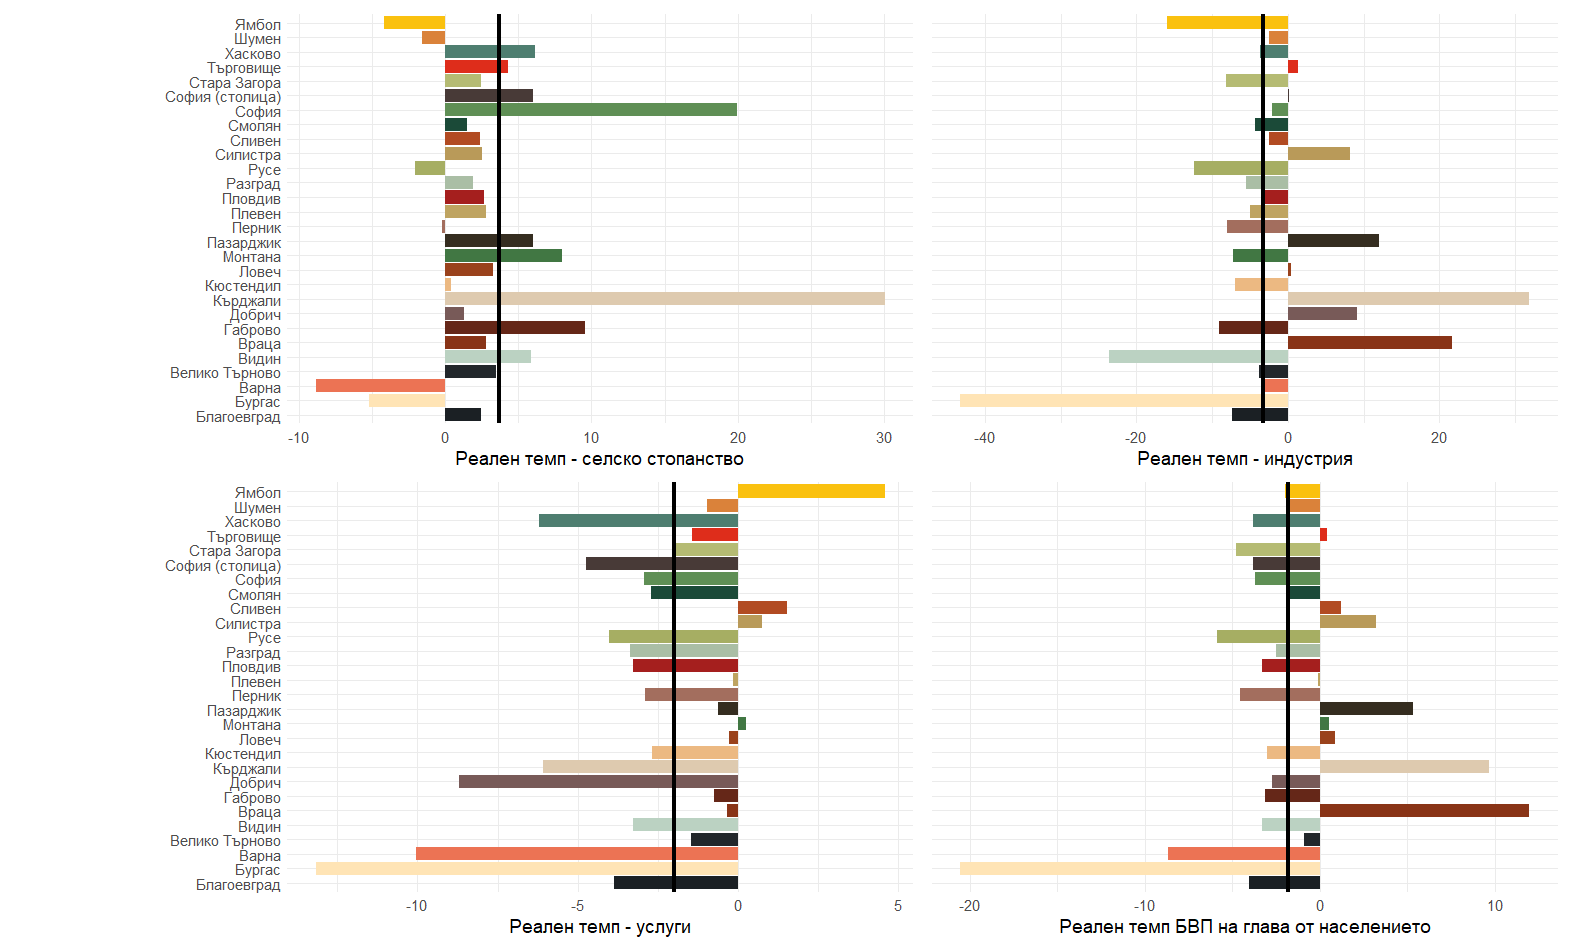
\includegraphics[width=1.45\textwidth, angle =90 ]{../graphics/gdpc_tem}
	\caption{Сравнителна характеристика на реалния темп на растеж: БВП на глава от населението, сектор селско стопанство, услуги и индустрия}
	\label{fig:gdpctem}
\end{figure}
\newpage



\newpage
\begin{figure}[H]

	\centering
	\hspace*{-2cm}
	\vspace*{-2 cm}
	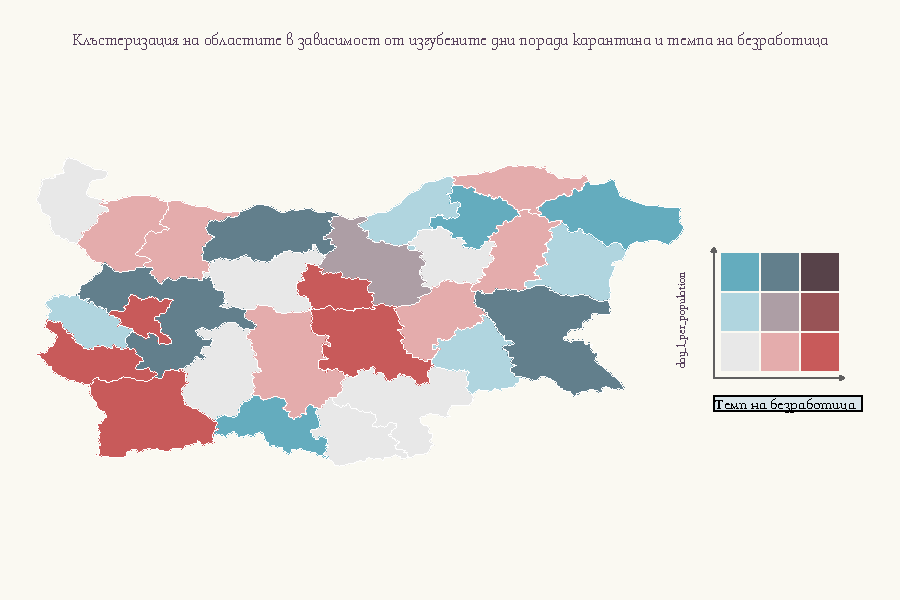
\includegraphics[width=1.5\textwidth,height= 20 cm, angle =90 ]{../graphics/Graph_2}
	\caption{{\scriptsize Клъстеризация на областите по факторите на редукция на работната сила- загубени дни поради карантина и темп на безработица}}
	\label{fig:graph2}
\end{figure}
\newpage

\subsection{Модел} 

Предвид изложените данни, се предположи влияние на факторите от страна на пандемията (заболеваемост, изгубени дни поради карантина), фактори от страна на противоепидемичните ограничения (затваряне на дейността в сектор услуги, намаляване на темпа на заетите и увеличаване на темпа на безработните) като основни тригери в намаляването на БВП на глава от населението. 

След тестване за колинеарност на факторите и приложение на линейна регресия (с robust оценка на стандартната грешка) се структурира 4 факторен модел на взаимодействие. 

\paragraph{БВП на глава от населението}.

В първия разработен модел се установява статистическа значими връзки с всички изследвани фактори. Позитивната разликата (2020-2019) в процентни пункта в използването на интернет сред населението в трудоспособна възраст е позитивно въздействащ фактор, като тези области с увеличена дигитализация се характеризират и с по-високи и позитивни стойности на темпа на изменение на БПВ на глава от населението. 

Изгубените дни поради карантина са сигнификатно повлияващ негативно реалния темп на растеж на БВП. Стандартизираният бета коефициент, установява като най-силно въздействащ фактор - темпа на изменение на броя заети на трудово правоотношение, като 1\% увеличение на този темп се асоциира с 1,92\% увеличение в темпа на реалния БВП на глава от населението. В селекцията на фактори този компонент е предпочетен заради високата колинеарност с коефициента на безработица и темпа на изменение на регистрираните в бюрата по труда.

Последният фактор определен като "пропорцията на жените в трудовата сила" и изразяващ съотношението "жени:мъже" в сред населението в трудова възраст, също е статистически значим, което може отчасти да се ползва за доказателство подкрепа и тезата за полови неравенства следствие на COVID - 19 пандемията. \cite{NBERw26947}


\begin{table}[H]
	\centering
	\caption{Модел за БПП на глава от населението}
	\begin{tabular}{lccccc}
		\toprule
		БВП на глава от населението  & Estimate & SE    & t     & p value & Stand. Beta \\
		\midrule
		(Intercept) & -35.84 & 15.14 & -2.37 & 0.03  &  \\
		Използване на интернет (\%) & 0.21  & 0.09  & 2.35  & 0.03  & 0.31 \\
		Изгубени дни поради карантина  & -0.01 & 0.00  & -3.71 & 0.00  & -0.37 \\
		Темп на заетите (трудово правоотношение) & 1.92  & 0.62  & 3.08  & 0.01  & 0.62 \\
		Пропорция на жените в трудоспобна възраст  & 99.05 & 32.48 & 3.05  & 0.01  & 0.39 \\
		\bottomrule
	\end{tabular}%
	\label{tab:addlabel}%
\end{table}%


\paragraph{Реален темп на изменение сектор Услуги}.

Разгледано изолирано приложен модела, само за реалния темп в сектор услуги=- згубените дни поради карантина загубват своето статистическо значение. Вероятна причина за това е, че сектора не е чувствителен на загуба на работна сила предвид пълното преустановяване на дейността в голяма част от него. Дори и работниците да бъдат заразени и карантинирани, това не би следвало да повлияе и потреблението на услугите поради невъзможността те да бъдат предоставени.

Същото е валидно и за фактора процент на жените в трудоспособна възраст. Основен и единствен значим статистически, остава темпа на изменение заетите, въпреки че по-сила се установява намален.

% Table generated by Excel2LaTeX from sheet 'Лист1'
\begin{table}[H]
	\centering
	\caption{Модел за реален темп за сектор Услуги}
	\begin{tabular}{lccccc}
		\toprule
		Реален темп - услуги & Estimate & SE    & t     & p value & Stand. Beta \\
		\midrule
		Използване на интернет (\%) & 0.05  & 0.07  & 0.80  & 0.43  & 0.12 \\
		Изгубени дни поради карантина  & 0.00  & 0.01  & 0.20  & 0.84  & 0.04 \\
		Темп на заетите (трудово правоотношение) & 1.39  & 0.39  & 3.56  & 0.00  & 0.70 \\
		Пропорция на жените в трудоспобна възраст  & 30.81 & 24.46 & 1.26  & 0.22  & 0.19 \\
		(Intercept) & -11.85 & 11.88 & -1.00 & 0.33  & . \\
		\bottomrule
	\end{tabular}%
	\label{tab:addlabel}%
\end{table}%

\paragraph{Реален темп на изменение сектор Индустрия}.

По отношение на сектор Индустрия, всички фактори в модела запазват своята статистическа значимост, като използването на интернет сред населението в трудоспособна възраст увеличава значително силата си. Това може да бъде обяснено със по-усилената дигитализация в сектора при съобразяване с противоепидемичните мерки, но без прекъсване на работния процес. 

За този показател е най-висок и нестандартизираният коефициент за темпа на заетите. Докато в сектор услуги 1\% увеличени в темпа на заетите се асоциира с 1,39 \%, за селско стопанство с 1,58 \% то за сектор Индустрия увеличението в реалния темп в отговор е 3,06 \%

\begin{table}[H]
	\centering
	\caption{Модел за реален темп за сектор Индустрия}
	\begin{tabular}{lccccc}
		\toprule
		Реален темп - индустрия & Estimate & SE    & t     & p value & Stand. Beta \\
		\midrule
		Използване на интернет (\%) & 0.68  & 0.23  & 2.91  & 0.01  & 0.43 \\
		Изгубени дни поради карантина  & -0.03 & 0.01  & -2.36 & 0.03  & -0.37 \\
		Темп на заетите (трудово правоотношение) & 3.06  & 1.83  & 1.67  & 0.11  & 0.42 \\
		Пропорция на жените в трудоспобна възраст  & 278.14 & 91.40 & 3.04  & 0.01  & 0.47 \\
		(Intercept) & -114.54 & 42.72 & -2.68 & 0.01  & . \\
		\bottomrule
	\end{tabular}%
	\label{tab:addlabel}%
\end{table}%


\paragraph{Реален темп на изменение сектор Селско стопанство}.

Разгледаните фактори в модела, не успяват да обяснят динамиката на реалния темп в селското стопанство. Единствения от секторите с позитивна стойност на реалният темп, въпреки невъзможността да компенсира във състава на БВП на глава от населението. 

Единствено темпа на изменение на заетите е със гранична статистическа стойност. Но въпреки това модела е със слаба обяснителна сила. Следва да се отбележи, че коефициентите в модела, приложени към различните сектори не сменят знака си. Това е косвен белег за липса на значими взаимодействия между самите фактори приложени за различните отрасли. 
\begin{table}[H]
	\centering
	\caption{Модел за реален темп за сектор Селско стопанство}
	\begin{tabular}{rccccc}
		\toprule
		\multicolumn{1}{l}{Реален темп - селско стопанство} & Estimate & SE    & t     & p value & Stand. Beta \\
		\midrule
		\multicolumn{1}{l}{Използване на интернет (\%)} & 0.24  & 0.16  & 1.51  & 0.14  & 0.28 \\
		\multicolumn{1}{l}{Изгубени дни поради карантина } & -0.02 & 0.01  & -1.59 & 0.13  & -0.41 \\
		\multicolumn{1}{l}{Темп на заетите (трудово правоотношение)} & 1.58  & 0.77  & 2.06  & 0.05  & 0.40 \\
		\multicolumn{1}{l}{Пропорция на жените в трудоспобна възраст } & 27.63 & 35.64 & 0.78  & 0.45  & 0.09 \\
		\multicolumn{1}{l}{(Intercept)} & 7.25  & 14.55 & 0.50  & 0.62  & . \\
		\midrule
		&       &       &       &       &  \\
	\end{tabular}%
	\label{tab:addlabel}%
\end{table}%


\section{Заключение}
Първата половина на 2020 г., е началото на новото нормално в икономически аспект. Непознатите предизвикателства в световната икономика, повлия сериозни и нашата страна, което е част от активната световна икономика. Оставането в глобалния пазар и адаптацията към новостите на светоната търговия са най-трудните задачи за всички икономически субекти.

Изводите, които могат да се направят от настоящия анализ на данни, показват ясно, че за 2020 г. икономиката на страната ни се свива непосредствено след въвеждането на противоепидемичните мероприятия. Секторите индустрия и услуги са сред най-засегнатите, като се характеризират със сходна факторна обусловеност. За Българската икономика на областно ниво -сектор "индустрия" е най-сериозно засегнат, въпреки "очакваните" последици върху сектор "услуги".

Съвкупното предлагане е ограничено в основа на два корелирани фактора- заболеваемостта и следствието от нея временно намалена работоспособност.

Вероятно е предположението, че ефектите от пандемията ще продължат да влияят негативно на икономическите процеси в нашата страна, което допълнено с политическата ситуация и необходимостта за увеличаване на сектор отбрана в световен мащаб ни води към задълбочаване на икономическата рецесия и охарактеризира възможна стагнация.



\bibliographystyle{vancouver}
\bibliography{reference}
\end{document}
